\section{Background}

Scientists for decades have studied the nuclear structures of various nuclei for their material properties, biological impacts, and natural origins. Further understanding of the nuclear structure has been a priority of the scientific community towards the development of innovative technology. In designing a spaceship, understanding the properties of shielding materials protects astronauts during space travel.

When a radioactive nucleus decays, it emits a radiation unique to the type of decay exhibited. Several radiation types and radioactive decays exist and shielding each type requires certain forms of sophistication. One decay scheme emits heavy charged particles, like an $\alpha$ particle:

\begin{equation}
{}^{A}_{Z}X \rightarrow {}^{A-4}_{Z-2}Y + {}^{4}_{2}{He}
\end{equation}

An $\alpha$ particle is a helium nucleus consisting of two neutrons and two protons. Since this is only a nucleus, it is positively charged relative to its surroundings. Because this is a large, charged particle, it has a very short range before interactions with its surroundings stop it. The $\alpha$ particle slows down either by collisions with other particles or by attractions with opposite charges that neutralize its own charge. Finding the range of heavy charged particles can be useful so that shielding the radiation can better be determined. With $\alpha$-decays, only a few centimeters of shielding may be required to protect against this harmful radiation, even when that shielding is simply air.

Another decay scheme is $\beta$-decays, in which a radioactive nucleus emits an electron or positron with an appropriate antineutrino:

\begin{equation}
{}^{A}_{Z}X \rightarrow {}^{A}_{Z+1}X + \beta^{-} + \bar{\nu_{e}}
\end{equation}

\begin{equation}
{}^{A}_{Z}X \rightarrow {}^{A}_{Z-1}X + \beta^{+} + \nu_{e}
\end{equation}

Where $\beta^{\pm}$ is just an electron or positron. Since this emission is a three-body problem, the $\beta$-particle can have a distribution of energies. $\beta$-particles are high energy can generally penetrate further than heavy-charged particles. Additionally, they can emit electromagnetic radiation as the $\beta$-particle deaccelerates called bremsstrahlung.

Some radioactive nuclei decay by emitting high energy electromagnetic radiation called $\gamma$-rays:

\begin{equation}
{}^{A}_{Z}X^{*} \rightarrow {}^{A}_{Z}X + {}^{0}_{0}\gamma
\end{equation}

In fact, nuclei may emit a large spectrum of electromagnetic radiation, not necessarily $\gamma$ radiation. Depending on the energy released, perhaps X-rays or ultraviolet radiation is released instead. Several interactions with materials can slow down $\gamma$ radiation \cite{krane}. Low energies are characterized by the photoelectric effect, in which $\gamma$ radiation is absorbed by an electron in the material, which is consequently freed by this new energy. Compton scattering occurs at medium energies, where the radiation collides with a target, imparting energy and changing the direction of both particles. At high energies (above 1022 keV) pair production dominates. This is where the $\gamma$ radiation turns into an electron-positron pair. The combination these interaction mechanisms results in radiation stopping power with slightly different characteristics than heavy charged particles like an $\alpha$ particle. Shielding performance of this radiation is characterized by an exponential decay \cite{knoll}:

\begin{equation}
I(t) = I_{0}e^{-\mu t}
\end{equation}

Here, $I_{0}$ is the radiation counting rate without an absorber, $t$ is the thickness of the absorber, and $\mu$ is the linear attenuation coefficient. $\mu$ is affected by the material uniqueness of the various interactions that stop $\gamma$ radiation. A mass attenuation coefficient ($\mu/\rho$) can also be defined that accounts for the density of a specific absorbing material \cite{knoll}:

\begin{equation}
I(t) = I_{0}e^{-(\frac{\mu}{\rho})\rho t}
\label{eq:decay}
\end{equation}

The coefficient can be experimentally determined and is unique to the shielding material. Of course, designing a shielding apparatus is not as simple as manipulating an exponential decay to within safe levels. As was demonstrated by bremsstrahlung, other radiation types can produce more radiation that has to be considered. Traditionally, this has resulted in engineers developing and using computer models that simulate the behavior of radiation in material types for designing an effective shield.

The dose absorbed in a mass (be it biological or a shield) is measured with the energy imparted by the radiation \cite{lamarsh}:

\begin{equation}
D = \frac{\Delta E_{D}}{\Delta m}
\end{equation}

In SI, this has the unit gray (Gy), which is 1 J/kg. More importantly, the biological dose can be calculated from this by weighting it with a quality factor, $Q$, or a weighting factor, $w_{R}$ \cite{lamarsh}:

\begin{equation}
H = D \times w_{R}
\end{equation}

\begin{figure}
\centering
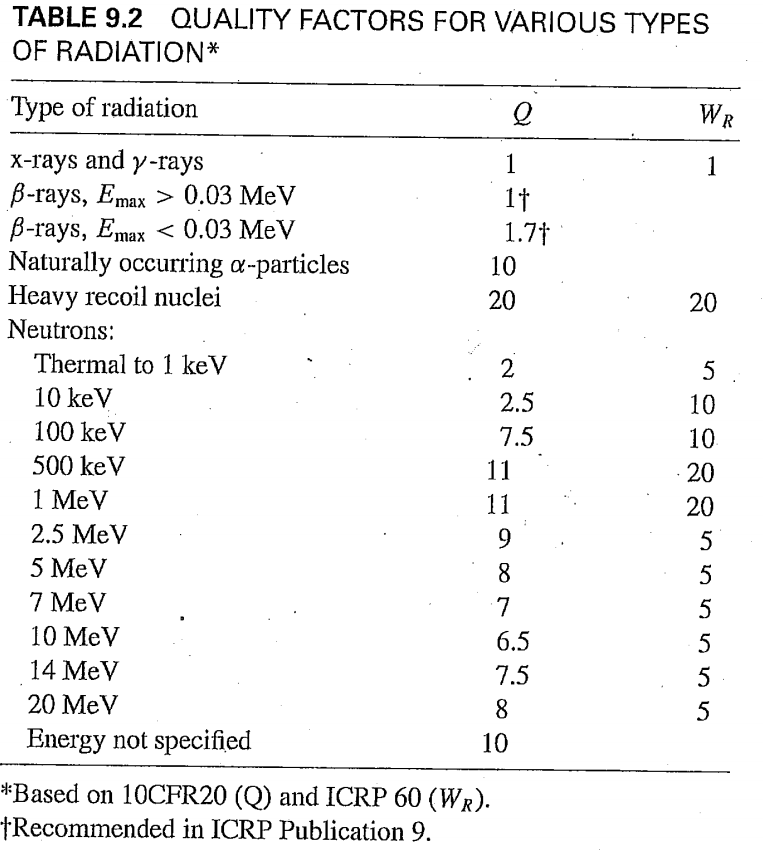
\includegraphics[width=\linewidth]{wr.png}
\caption{As presented in \cite{lamarsh}. Several quality and weighting factors are lsited for different types of radiation and radiation energies. These values can also be tabulated for different organs. These values are determined from the LET of each radiation.}
\label{fig:wr}
\end{figure}

The unit here is the sievert. 1 Sv = 100 Gy (affected by the weighting). These weighting factors are determined from the linear energy transfer (LET) of different radiation types. See Fig. \ref{fig:wr} for a catalog of factors determined for different radiation types. These weighting factors can also be organized by type organ in which the radiation is deposited. A limit for humans can then be determined from the effective dose received by all organs. Engineers strive to design vessels with enough shielding to prevent astronauts from exceeding this limit while still being operable and economical.
